5\documentclass[a4paper, 12pt, french, twoside]{article}
\usepackage{graphicx,wrapfig,lipsum}
\usepackage{graphicx}
\usepackage{mathtools}
\usepackage{amsmath}
%\frenchbsetup{StandardLists=true} à inclure si on utilise 
\usepackage[french]{babel}
\usepackage{enumitem}
\usepackage{float}
%\usepackage[top=2.5cm, bottom=2cm, left=2cm, right=2cm, showframe]{geometry}
\usepackage[top=2.5cm, bottom=2cm, left=2cm, right=2cm]{geometry}
\usepackage{caption}
\usepackage{amsmath}
\usepackage{graphicx} % Required for inserting images
\usepackage{subcaption}
\usepackage{hyperref}
\usepackage{makecell}
\usepackage{amsfonts}
\usepackage{amsthm}


\newtheorem{theorem}{Théorème}[section]
\newtheorem{corollary}{Corollaire}[theorem]
\newtheorem{lemma}[theorem]{Lemme}
\newtheorem{proposition}{Proposition}[theorem]
\newtheorem{defi}{Définition}[theorem]
\newtheorem{rem}{Remarque}[theorem]

\usepackage{pdfpages} % lien Pdf test
 \usepackage{tcolorbox}

\usepackage{cleveref}
\crefrangelabelformat{equation}{(#3#1#4--#5#2#6)}
\crefname{equation}{Eq.}{Eqs.}
\Crefname{equation}{Equation}{Equations}


%\usepackage{movie15}
\usepackage{epstopdf}
\usepackage{subcaption}
\usepackage{multicol}

%a abréviations
\def \be {\begin{equation}}
\def \ee {\end{equation}}
\def \dd  {{\rm d}}
\def \bm {\begin{pmatrix}}
\def \em {\end{pmatrix}}

%Ensembles 
\newcommand{\Cc}{{\mathbb{C}}}
\newcommand{\Ct}{\Cc^\times}
\newcommand{\Hh}{{\mathbb{H}}}
\newcommand{\Nn}{{\mathbb{N}}}
\newcommand{\Zz}{{\mathbb{Z}}}
\newcommand{\Zzn}{\Zz/n\Zz}
\newcommand{\ZzNt}{(\Zz/N\Zz)^\times}%quotient 
\newcommand{\Rr}{{\mathbb{R}}}
\newcommand{\Rt}{{\Rr^\times}}
\newcommand{\Qt}{{\Qq^\times}}
\newcommand{\Qq}{{\mathbb{Q}}}
%to do later
\newcommand{\later}[1]{\textcolor{orange}{[#1]}}
\newcommand{\com}[1]{\textcolor{magenta}{[#1]}}

%to make hyper refs not surrounded with red
\hypersetup{pdfborder=0 0 0}
\hypersetup{
    colorlinks=true,
    linkcolor=blue,
    filecolor=magenta,      
    urlcolor=cyan,
    pdftitle={Overleaf Example},
    pdfpagemode=FullScreen,
    }
    
\title{Corrigé 2}

\begin{document}

\maketitle

% \section{Exo (Gaétan) \textbf{A VERIFIER, PAS SUR DE MOI}}
% Montrer par contradiction qu'une suite de Cauchy est bornée.

% Donc il s'agit de montrer qu'une suite non bornée n'est pas de Cauchy. Si une suite n'est pas bornée, cela implique qu'elle tend vers $\pm \infty$. Sans perdre de généralité, posons la suite $(x_n)$ telle que 
% \begin{equation*}
%     \lim_{n\rightarrow\infty}x_n=+\infty
% \end{equation*}

% Ainsi, posant $m\in \Nn$ fixée, on observe que :

% \begin{equation}
%     lim_{n\to\infty}|x_n-x_m|=\infty.
% \end{equation}
% Cette suite ne peut donc pas obéir à l'inégalité présente dans la définition d'une suite de Cauchy. Ainsi, une suite non bornée ne peut être de Cauchy ce qui implique qu'une suite de Cauchy est bornée. 

% \section{Exo Gaétan}
% Puisque $(x_n), n\in \Nn$ est bornée supérieurement, il existe $b = sup\{x_n ; n \in \Nn\}$ . Maintenant, par définition du supremum, on a que $\forall \varepsilon > 0$ , $∃ ñ$ tel que $b - \varepsilon \leq x_{ñ }\leq b$ .

% Mais $(x_n)$ est croissante et on a donc
% \begin{equation}
%     b - \varepsilon \leq x_{ñ} \leq x_{ñ+1} \leq ... \leq b ,    
% \end{equation}

% et ainsi $lim_{n\to \infty}
% x_n = b = sup\{x_n ; n \in \Nn\}$ .

\section{Limites usuelles}

\begin{enumerate}
    \item Pour $x_n=n$: \\
    On observe trivialement qu'elle tend vers l'infini. Pour le démontrer facilement, il suffit de montrer qu'elle est croissante et non bornée. La croissance est évidente. Pour la bornée, si l'on suppose qu'elle est bornée par un nombre $k\in \Rr$, alors on observe que $x_{k+1}>k$. Ainsi elle n'est pas bornée et est croissante: elle diverge vers l'infini.
    \item Pour $x_n=n^p$, $p>0$: \\
    Démontrons qu'elle tend vers l'infini. Premièrement elle est croissante. De plus, si l'on suppose qu'elle est bornée par un nombre $k\in \Rr$, alors on observe que $x_{t}>k$, $t=(k+1)^\tfrac{1}{p}c$. Ainsi elle n'est pas bornée et est croissante: elle diverge vers l'infini.
    \item Pour $x_n=n^p$, $p\leq0$: \\
    Si $p=0$, on a $x_n=1$ donc la limite est 1.
    Pour $p<0$, démontrons qu'elle tend vers 0. Il est possible de le faire en montrant qu'elle est bornée par 0 et décroissante. Autrement, en appliquant le définition, trouvons le rang $N$ pour un $\varepsilon>0$ fixé tel que $|x_N|<\varepsilon$.
    $|x_N|<\varepsilon \iff N^p<\varepsilon \iff \frac{1}{\varepsilon}<N^{|p|}\iff \left( \frac{1}{\varepsilon}\right)^{\tfrac{1}{|p|}} <N $. Nous avons trouvé un rang à partir duquel la propriété est vraie. La suite tend bien vers 0.
    \item Pour $x_n=a n^p$:\\
    Si $a=0$, la suite vaudra 0 donc admet 0 comme limite. Sinon, si $p=0$ la suite vaut $a$ et l'admet donc comme limite. Sinon, si $p$ est négatif, la suite tend vers 0 comme vu à travers de l'exercice précédent. Si $p$ est positif, la suite tend vers $\text{sgn}(a) \infty$.
    \item Pour $x_n=\frac{n^p}{n^q}$:\\
    On a $x_n=n^{p-q}$ et retournons à la question précédente et observons que cela dépend du signe de $p-q$.
    \item Pour $x_n=\dfrac{a_pn^p+a_{p-1}n^{p-1}+...+a_0}{b_qn^q+b_{q-1}n^{q-1}+...+b_0}$:\\
    Nous allons utiliser les précédentes règles démontrées. Premièrement, $x_n=\dfrac{a_pn^p}{b_qn^q}\cdot\dfrac{1+\sum_{k=1}^{p-1} \frac{a_k}{a_p}n^{k-p}}{1+\sum_{k=1}^{q-1} \frac{b_k}{b_q}n^{k-q}}$. La fraction de droite tend vers 1 car chaque somme tend vers 0 de par le fait que $p-k$ et $q-k$ sont toujours négatifs. Ainsi, on a $lim_{n\to\infty} x_n=lim_{n\to\infty} \dfrac{a_pn^p}{b_qn^q}=\dfrac{a_p}{b_q}lim_{n\to\infty} \dfrac{n^p}{n^q}$ que l'on a démontré dans la question précédente.  
\end{enumerate}



\section{Sous-suites, Principe des deux gendarmes}

\subsection{Sous-suites}

\textbf{a)} \\

\begin{figure}[H]
    \centering
    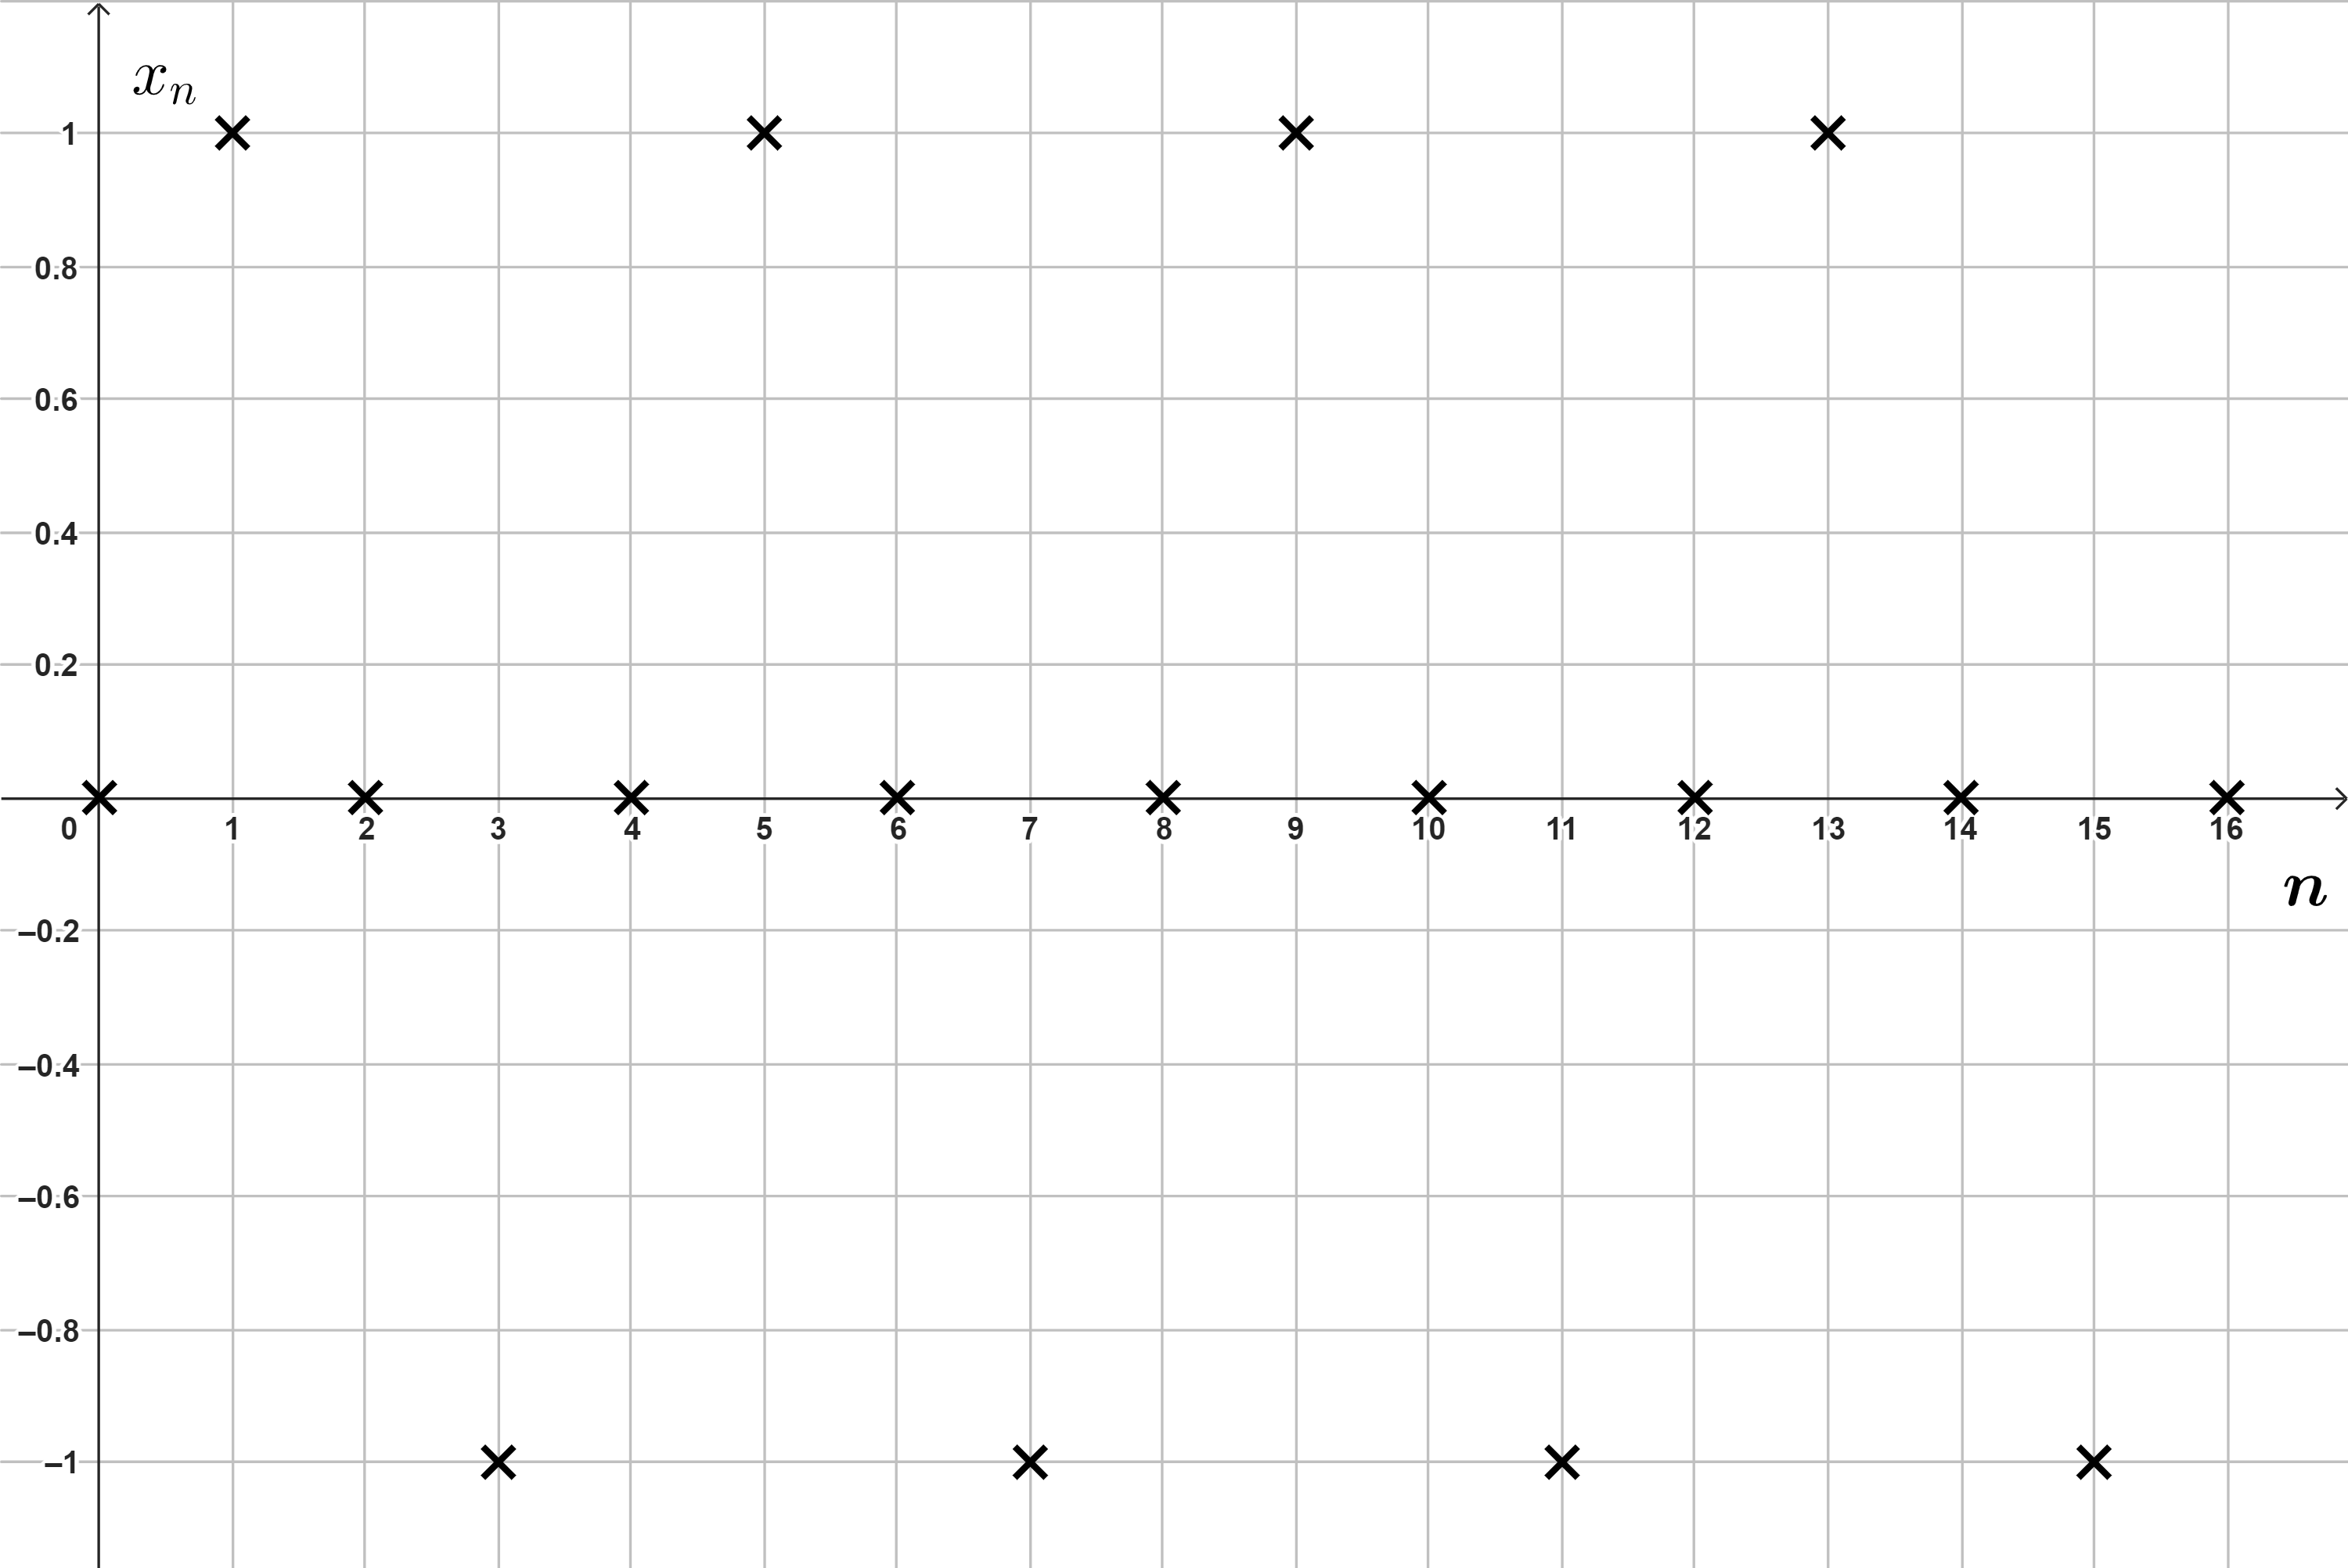
\includegraphics[scale=0.7]{Exercices/schema2.png}
    \caption{Representation des premiers termes de la suite $x_n=sin(n\frac{\pi}{2}$.}
    \label{fig:enter-label}
\end{figure}

\textbf{b)} La suite $x_n$ ne converge pas, mais la sous-suite $x_{2n}$ converge vers 0 (elle est d'ailleurs même constante: elle vaut toujours 0).\\

\textbf{c)} Pour rappel, les limites inférieure et supérieure d'une suite sont respectivement l'infimum et le suprémum des limites des sous-suites de $x_n$. Notre dessin au point \textbf{a)} nous montre que la limite inférieure est de -1 (obtenue par exemple avec la sous-suite $x_{1+4n}$) et la limite supérieure de 1 (obtenue par exemple avec la sous-suite $x_{3+4n}$). \\

\textbf{d)} La suite converge vers 0. \\


\begin{figure}[H]
    \centering
    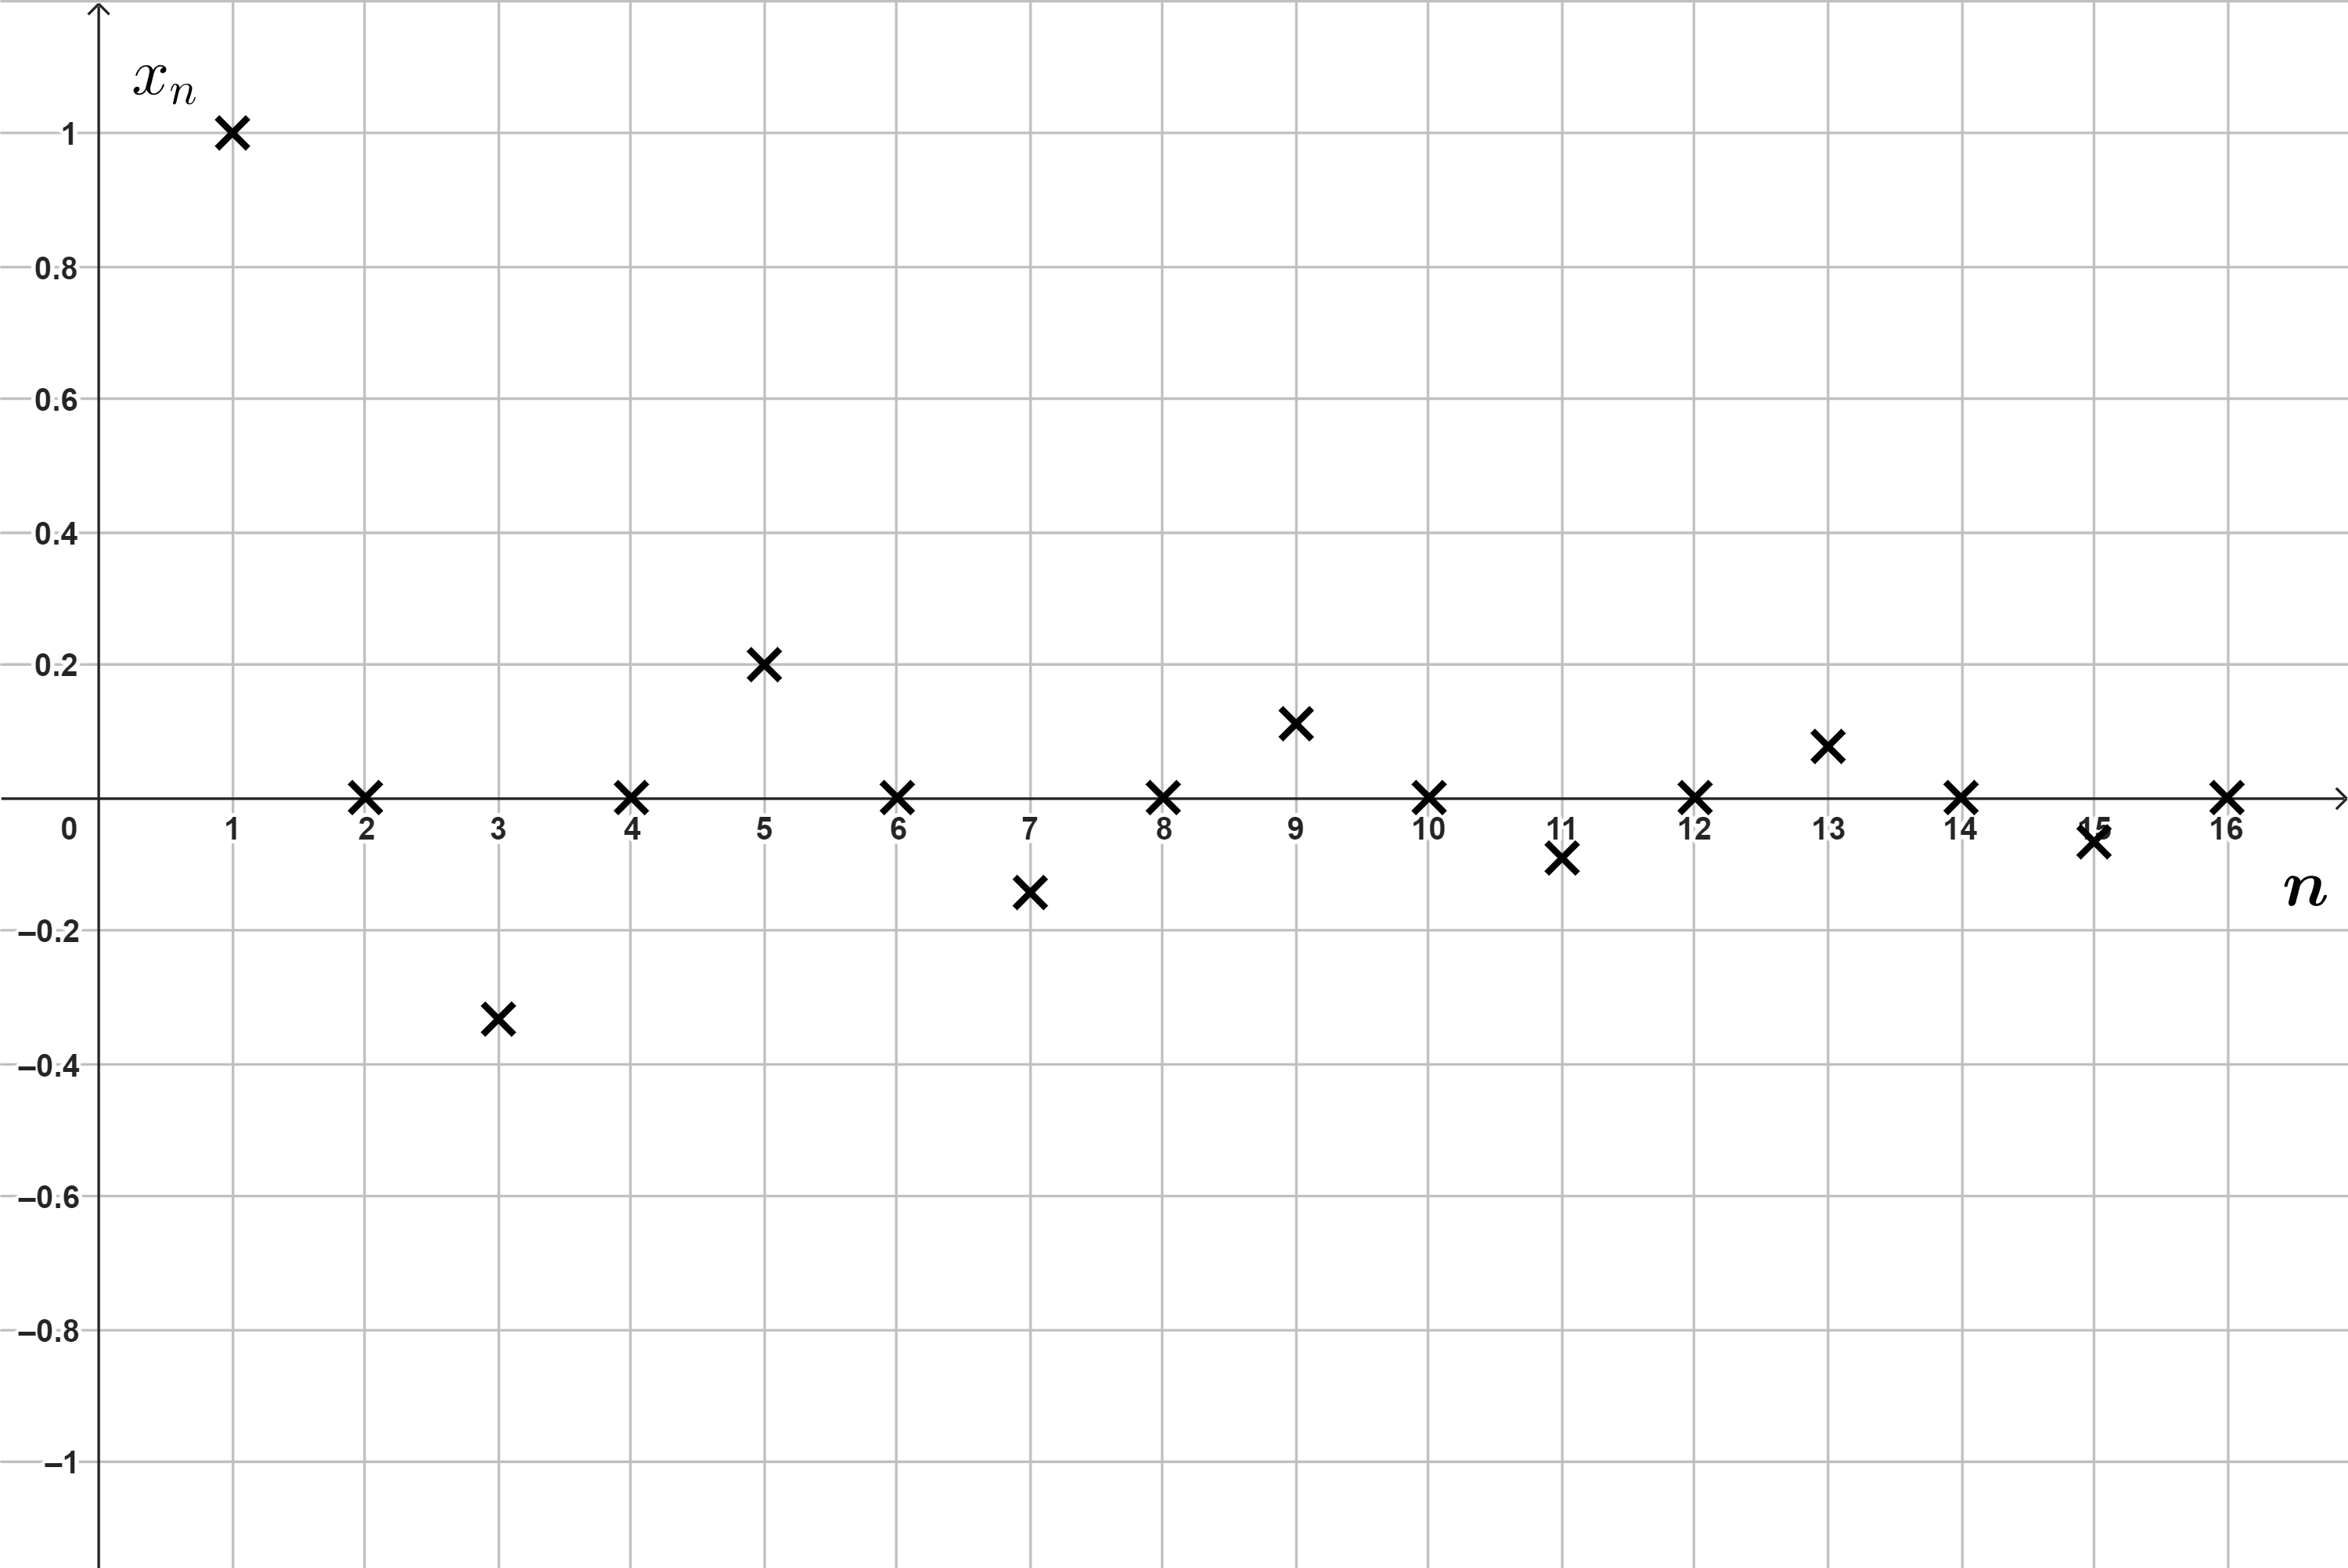
\includegraphics[scale=0.7]{Exercices/schema3.png}
    \caption{Representation des premiers termes de la suite $x_n=\frac{sin(n\frac{\pi}{2}}{n}$.}
    \label{fig:enter-label}
\end{figure}

\textbf{e)} Non. Il suffit de reprendre la définition de limite de suite pour s'en convaincre. Supposons qu'une suite $x_n$ converge vers $l$. On sait alors que quelque soit le $\epsilon$, on peut trouver un $N$ tel que $n \geq N \Rightarrow |x_n - l| < \epsilon$. \\
Pour rappel, une sous-suite est définie par $x_{n_k}$ avec $n_k = \phi(k), \ \forall k \in \Nn$, où $\phi: \Nn \rightarrow \Nn$ est une fonction strictement croissante. La suite des $n_k$ étant strictement croissante, on sait que pour tout $N$ qui satisfait $n \geq N \Rightarrow |x_n - l| < \epsilon$ dans la suite originale $x_n$, on pourra trouver un $K$ tel que $k \geq K \Rightarrow n_k \geq N$ et donc $|x_{n_k} - l| < \epsilon$.

\subsection{Principe des deux gendarmes}

\textbf{a)} On peut par exemple prendre $v_n = -\frac{1}{n}$ et $w_n = \frac{1}{n}$, car $-1 \leq sin(\frac{n \pi}{2}) \leq 1$. \\

\textbf{b)} Puisque $\lim_{n\rightarrow\infty}v_n=\lim_{n\rightarrow\infty}w_n=l$, on peut trouver $n_0\in\Nn$, tel que:
\begin{equation*}
    v_n-l>-\varepsilon \quad et \quad w_n-l<\varepsilon, \quad \forall n \geq n_0.
\end{equation*}
Alors on a 
\begin{equation*}
    -\varepsilon<v_n-l\leq y_n-l \leq w_n-l < \varepsilon, \quad \forall n \geq n_0,
\end{equation*}
et ainsi $\lim_{n\rightarrow\infty}y_n=l.  $ \\

\faLightbulbO \quad \fbox{\textbf{Discutez}} Il est plus facile de commencer par borner le dénominateur dans le présent exemple:
\begin{equation}
    n-1 \leq n + sin(n) \leq n+1 \Rightarrow \frac{1}{n+1} \leq \frac{1}{n + sin(n)} \leq \frac{1}{n-1},
\end{equation}
où on utilise le fait que l'inversion des members d'une inéquation change le sens de l'inégalité à condition que les membres soient positifs.

\section{Suite de Cauchy}

\textbf{a)} Pour $n,m \geq 1$, l'inégalité triangulaire donne:
\begin{equation}
    |x_n - x_m| = \Bigl\lvert\frac{(-1)^n}{n} - \frac{(-1)^m}{m}\Bigl\rvert \leq \frac{1}{n} + \frac{1}{m},
\end{equation}
ce qui montre que $x_n$ est une suite de Cauchy. En effet, pour un $\epsilon$ donné, prenons $N \in \Nn$ tel que $N > 2/\epsilon$. Alors,
\begin{equation}
    |x_n - x_m| \leq \frac{1}{n} + \frac{1}{m} \leq \frac{\epsilon}{2} + \frac{\epsilon}{2} = \epsilon, \quad \forall n,m \geq N.
\end{equation}
\\


\begin{figure}[H]
    \centering
    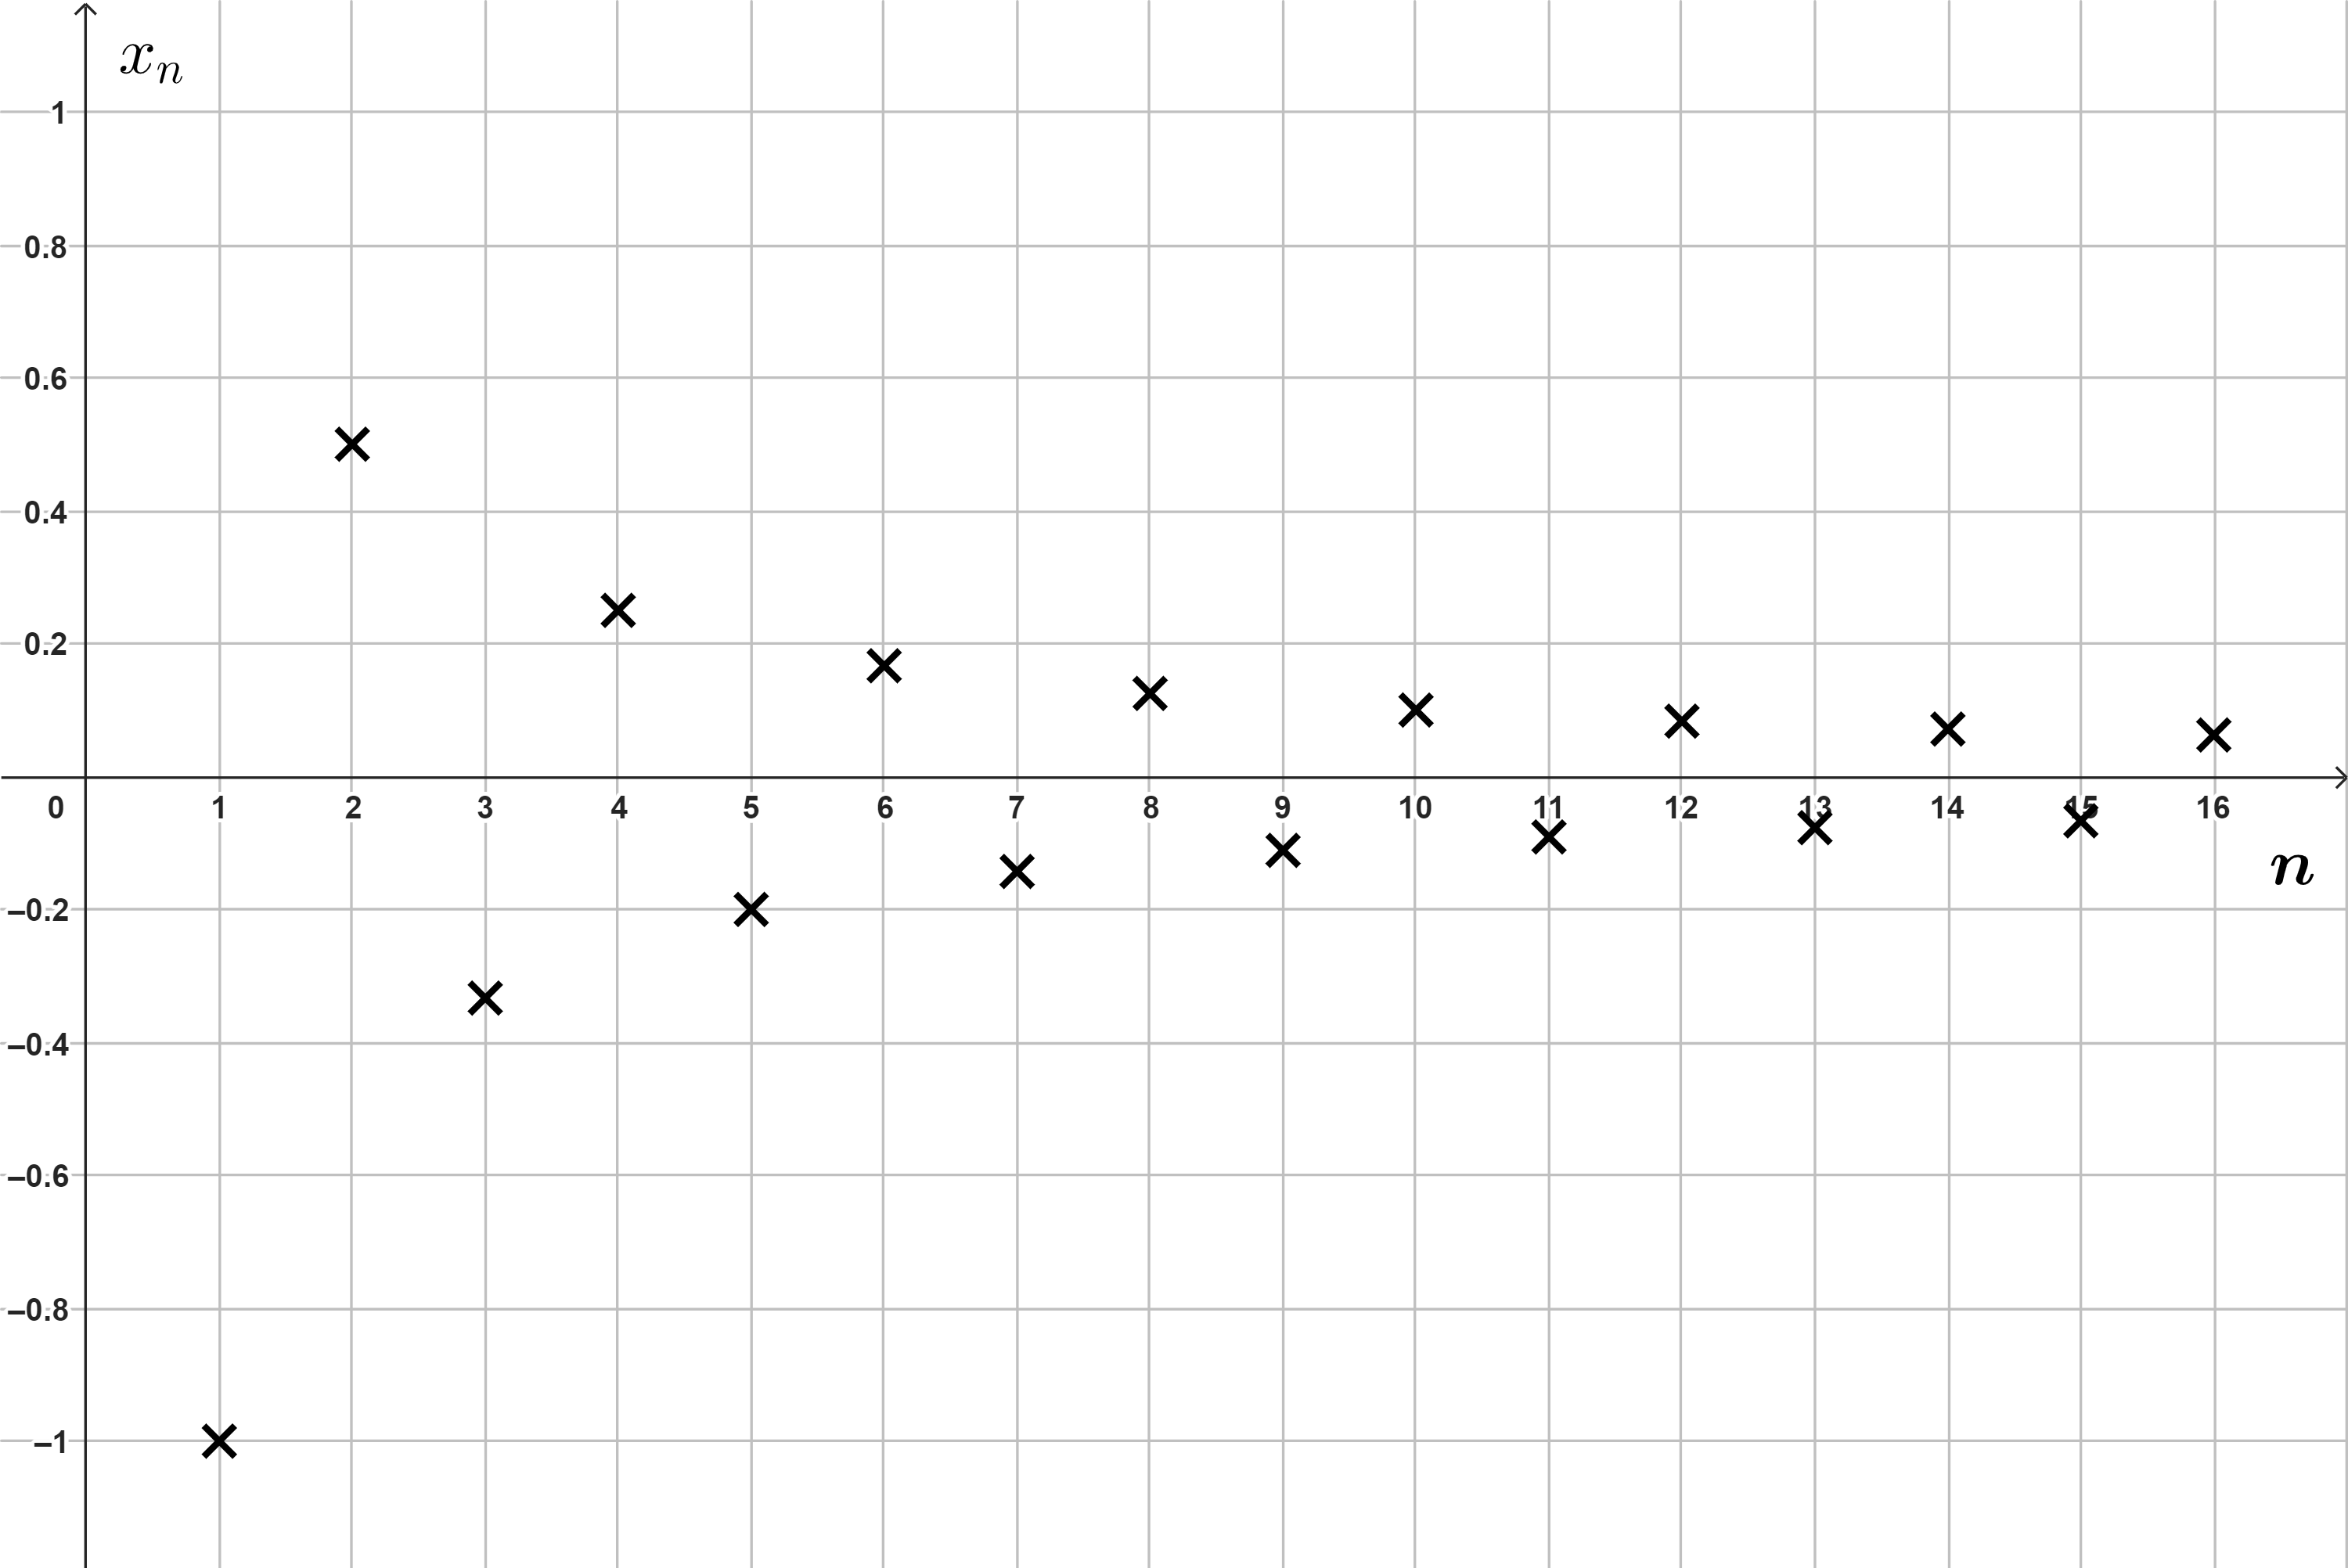
\includegraphics[scale=0.7]{Exercices/schema4.png}
    \caption{Representation des premiers termes de la suite $x_n=\frac{(-1)^n}{n}$}
    \label{fig:enter-label}
\end{figure}

\textbf{b)} Comme indiqué dans l'indice, il s'agit de montrer qu'une suite non bornée n'est pas de Cauchy. Si une suite n'est pas bornée, cela implique qu'elle tend vers $\pm \infty$. Sans perdre de généralité, posons la suite $(x_n)$ telle que 
\begin{equation*}
    \lim_{n\rightarrow\infty}x_n=+\infty.
\end{equation*}

En posant un $m\in \Nn$ fixe (par exemple $m=0$), on observe que :

\begin{equation}
    lim_{n\to\infty}|x_n-x_m|=\infty.
\end{equation}
Ceci entre en contradiction avec l'inégalité présente dans la définition de suite de Cauchy, qui doit être respectée quelle que soit la valeur de $m$. \\
On vient donc de montrer qu'une suite non bornée ne peut pas être de Cauchy. Par conséquent, toute suite de Cauchy est forcément bornée. \\

\faLightbulbO \quad \fbox{\textbf{Discutez}} Non. Notons la proposition ``la suite est de Cauchy" A, et la proposition ``la suite est bornée" B. L'affirmation à prouver est donc $A \Rightarrow B$, soit en français ``si A est vrai, alors B est forcément vrai aussi". \\
Cette affirmation est équivalente à ``si B est faux, alors A est forcément faux aussi": $\neg B \Rightarrow \neg A$, où $\neg$ est le symbole de négation. On pourrait lire cela ``si B est faux alors le contraire de A est vrai", soit ``si suite bornée est faux (suite non bornée), alors le contraire de suite de Cauchy (la contradiction de suite de Cauchy, d'où le nom de démonstration par contradiction) est vrai".\\
Ce n'est en revanche pas équivalent à ce qui est proposé dans cet exercice: $\neg A \Rightarrow \neg B$ (soit ``si A est faux, alors B est forcément faux aussi") n'est pas équivalent à $A \Rightarrow B$!


\end{document}

